\documentclass[conference]{IEEEtran}
\IEEEoverridecommandlockouts
% The preceding line is only needed to identify funding in the first footnote. If that is unneeded, please comment it out.
\usepackage{cite}
\usepackage{amsmath,amssymb,amsfonts}
\usepackage{graphicx}
\usepackage{textcomp}
\usepackage{xcolor}
\def\BibTeX{{\rm B\kern-.05em{\sc i\kern-.025em b}\kern-.08em
    T\kern-.1667em\lower.7ex\hbox{E}\kern-.125emX}}

%%%%%%%%%%%%%%%%%%%%%%%%%%%%%%%%%%%%%%%%%%%%%%%%%%%
\usepackage[pdftex]{hyperref}


\usepackage{subcaption}
\usepackage{pdflscape}
\usepackage{pdfpages}
\usepackage{float}
\usepackage{multirow}
\usepackage[nottoc]{tocbibind}
\usepackage{afterpage}
\usepackage{tikz, lipsum,lmodern}
\usepackage{calligra,frcursive,xcolor}
\usepackage{pifont}
\usepackage[most]{tcolorbox}
\usepackage{fancyvrb}
\usepackage{array}
\usepackage{tabularx}
\usepackage{multirow}
\usepackage{pgfplots}
\usepackage{algpseudocode}
\usepackage{algorithm}
\usepackage{algorithmicx}
\usepackage{ulem}
 \usepackage{booktabs} 
\definecolor{myYellow}{HTML}{EDBB00}
%%%%%%%%%%%%%%%%%%%%%%%%%%%%%%%%%%%%%%%%%%%%%%%%%%%
\usepackage{todonotes}
\newcommand{\revL}[1]{\textcolor{blue}{#1}}
\newcommand{\revR}[1]{\textcolor{myYellow}{#1}}
\newcommand{\revJ}[1]{\textcolor{red}{#1}}
\newcommand{\todoL}[1]{\todo[inline,color=blue]{LEO: #1}}
\newcommand{\todoR}[1]{\todo[inline,color=myYellow]{RICARDO: #1}}
\newcommand{\todoJ}[1]{\todo[inline,color=purple]{JAVI: #1}}
%%%%%%%%%%%%%%%%%%%%%%%%%%%%%%%%%%%%%%%%%%%%%%%%%%%%%%
\begin{document}

\title{A probabilistic learning-based routing scheme with path planning of autonomous agricultural vehicles for assisted harvesting tasks\\
\thanks{Identify applicable funding agency here. If none, delete this.}
}

\author{\IEEEauthorblockN{1\textsuperscript{st} Ricardo Urvina Córdova}
\IEEEauthorblockA{\textit{Universidad Católica del Norte} \\
\textit{Antofagasta, Chile} \\
ricardo.urvina@alumnos.ucn.cl}
\and
\IEEEauthorblockN{2\textsuperscript{nd} Leonardo Guevara}
\IEEEauthorblockA{\textit{Lincoln Institute for Agri-Food Technology} \\
\textit{Lincoln Centre for Autonomous Systems} \\
\textit{University of Lincoln, UK} \\
lguevara@lincoln.ac.uk}
\and
\IEEEauthorblockN{3\textsuperscript{rd} Alvaro Prado}
\IEEEauthorblockA{\textit{Universidad Católica del Norte} \\
\textit{Antofagasta, Chile} \\
alvaro.prado@ucn.cl}
}

\maketitle
%%%%%%%%%%%%%%%%%%%%%%%%%%%%%%%%%%%%%%%%%%%%%%%%%%%%%%

\begin{abstract}
\textcolor{blue}{This article presents a combined route and path planning strategy to guide autonomous ground vehicles in scheduled harvest tasks within expansive crop rows subject to complex terrain conditions of agricultural fields. The proposed planning strategy integrates i) a global planning method based on the Traveling Salesman Problem under the Capacitated Vehicle Routing approach to prioritize harvesting positions according to criteria of minimum path length and vehicle's load capacity, and ii) a local planning strategy based on Informed Rapidly-exploring Random Trees (IRRT$^*$) to coordinate the previously scheduled harvesting points while simultaneously avoiding obstacles of low-traction terrain. The global approach aims to generate an ordered queue of harvesting locations, maximizing the amount of harvested product of the expected crop yield. On the other hand, in the second stage, the IRRT$^*$ planner avoids potential obstacles, including the agriculture farm layout and slippery terrain conditions. To do so, it is incorporated a traversability model and a dynamical model of the vehicle motion dynamics to meet constraints compatible with those of the planned path. Experimental results demonstrated the effectiveness of the proposed planning strategy, achieving smooth and collision-free paths, making it suitable for practical applications in precision agriculture}.  
\end{abstract}

\begin{IEEEkeywords}
Path planning, Travel salesman problem, rapidly exploring random trees, capacitated vehicle routing, \revL{agricultural ground vehicles}.
\end{IEEEkeywords}
%%%%%%%%%%%%%%%%%%%%%%%%%%%%%%%%%%%%%%%%%%%%%%%%%%%%%%

\section{Introduction}
\textcolor{blue}{The Food and Agriculture Organization (FAO) forecasts that by 2030, a 70\% increase in agricultural productivity will be necessary to sustain the growing global population of nearly 9 billion people. \cite{FAO2050}. To meet these new demands while adhering to stringent quality standards in the global markets, the digital farming has become the prevailing path for the future agricultural development. Then, increasing agricultural productivity through the adoption of technological advances is currently contributing to the fulfillment of such goals \cite{Prado2018}. For instance, the agriculture process will require autonomous mobility to assist in primary tasks such as tillage, watering, sowing, fertilizing, and spraying, as well as central tasks such as supervising, hauling, and harvesting, among others. All of these tasks will require agricultural ground vehicles capable of autonomously planning their tasks and routes}.

\textcolor{blue}{The process of manual harvesting in farmlands has typically relied on human labor and traditional farm equipment. The workers have generally operated machines or tools in the agricultural process to guide reap crops, such as fruits, vegetables, or grains, and then gather them for further processing. Such agricultural process is labor-intensive, time-consuming, and can be physically demanding. Furthermore, it relies on the expertise of farm workers to determine the optimal picking and collection time, preference harvesting locations, quantity of product collection, and quality in product sorting. This challenging process, though operationally straightforward, encompasses several concerns. The first shortcoming is that crop production can vary significantly between rows due to varied soil quality, sunlight exposure, and other environmental aspects. This makes it difficult to plan the assignment of workers to the highest-yield areas. Similarly, harvesting perishable and fragile products that are subject to unpredictable weather and environmental conditions, such as fruits or vegetables, could jeopardize both the quantity and quality of the harvested product, requiring timely collection. Hence, it is appealing to conceive routing and path planning techniques for autonomous ground vehicles that prioritize harvesting locations based on closeness to harvesting points of maximum crop yield.}

\textcolor{blue}{One of the key aspects to enhance the product collection process is the execution of planning strategies that consider the optimal sequence of multiple harvesting locations and navigation points \cite{GUEVARA2021, s21237898}. Furthermore, optimizing product harvest in agriculture entails the efficient implementation of path-planning strategies that set appropriate sequences for coordinating harvest locations, where either manual or autonomous vehicles attend to the crop harvest by quickly positioning themselves near these harvest points. For example, global planners, such as those focused on the Traveling Salesman Problem (TSP), usually compute combination sequences ordered for the shortest route according to specific navigation objectives \cite{9896838, GRAFPLESSEN201999}. However, a combined local path planning is usually required to guide the autonomous vehicle between global harvesting points, as proposed in this work. Beyond the conceptual simplicity of TSP, various methods such as those based on the vehicle routing problem \cite{HE2019387, 2034192}, ant colony optimization \cite{agriculture12070986, 12132}, genetic algorithms \cite{1729881420925310}, and others using heuristics have also been aimed at exploring ordered routes of minimum traveling proximity and time (see \cite[and their reference therein]{Yahia2023}). In practice, TSP-based methods, addressing further than route travel optimization, can directly impact vehicle resource utilization, obstacle avoidance, load motion capacity, traversability, and energy efficiency when integrated to local planners, as proposed in this study \cite{Planas, Janos2021}}. 

\textcolor{blue}{The efficient local planning of feasible and adaptable paths is crucial for navigating environments with static and dynamic obstacles. Local path planning methods primarily target the avoidance of predicted obstacles or the fulfillment of structural characteristics within workspace maps \cite{Pak2022, Tagliavini2022, Gan2018, 8715479}. However, there are not enough practical approaches that integrate requirements of priority points in harvesting maps, all while considering obstacles and terrain traversability. This gap highlights a critical problem in the existing methods, as exemplified by sampled-based approaches such as Dijkstra, A$^*$, or Probabilistic Road Mapping (PRM) \cite{Xu2020}, to name a few. Although these methods aim at finding the shortest path length toward reachable goals, they often neglect aspects such as motion dynamics feasibility, crop workspace layout, and terra-mechanical constraints because of inherent complexity of the environment. Therefore, these methods do not assure the generation of kinematically compatible paths with the robot's motion dynamics. To address such limitations, probabilistic techniques focused on Rapidly-exploring Random Trees (RRT) \cite{Mashayekhi2020, Kontoudis2019,Zhang2019,Denggui} are often used for path planning subject to robot's kinematic constraints. These RRT techniques offer a potential solution to the challenge of exploring feasible paths in complex search workspaces \cite{Xie2020}. Their variants have been demonstrated to be capable of being integrated with global path planners and suitable for generating feasible paths that consider motion models and terrain traversability criteria, which comprises the main reason why using probabilistic approaches based on RRT here in this study.}

\revJ{FAVOR, NO TOPAR LO AZUL}

\textcolor{blue}{The main contribution of this study is an integrated path-planning method composed of a global and a ocal planning strategy for assisted harvesting tasks in agricultural scenarios. The proposed global route planning approach is based on the TSP strategy for scheduling the harvested locations underlying insights of the CVRP approach to account for navigation objectives and constraints, whereas the local path planning uses a designed Informed Rapidly-exploring Random Tree star (IRRT$^*$) approach. The proposed path planning strategy is able to generating kinematically feasible paths for Skid-Steer Mobile Robot (SSMR) dynamics that further account for the vehicle payload capacity and terrain traversability criteria. Briefly, the key aspects of this research are:}

\begin{itemize}
    \item \textcolor{blue}{A global path planning called TSP-CVRP that is formulated as an integrated TSP and CVRP strategy that prioritizes the harvest points according to vehicle payload capacity constraints versus closeness between crop harvest locations}.
    \item \textcolor{blue}{A local path planning coordinated with a global one that explores scheduled harvesting waypoints based on IRRT$^*$ to achieve feasible and kinematically compatible paths with SSMR dynamics, accounting for obstacle avoidance and terrain traversability posed by low-traction surfaces}.
\end{itemize}

\textcolor{blue}{Beyond other planners that only consider the minimization of path length and disregard the agricultural production process, the proposed work also considered predicted crop yield maps with multiple harvesting locations among farm aisles to determine the priority between navigation points until reaching storage terminals, sorting areas, or packing zones characterized by terminal spots. In addition to obstacle avoidance and minimizing closeness between waypoints, the structural constraints of crop rows are taken into account here, requiring the path to appropriately border each row. The proposed strategy is capable of planning and re-planning paths as full load or unforeseen obstacles are detected to avoid harvest exposure to the environment, which is expected to improve product quality. The proposed strategy preliminary considers an environment map rendered as an RGB image, and then such an image is processed to provide a tailored scenario deployed for the local planner. Then, taking advantage of information about the current harvest positions and product quantity to be harvested for each row, the TSP-CVRP strategy schedules a navigation path, containing a queue list of prioritized harvest points by maximizing the load capacity of the SSMR. The resulting ordered list of harvesting points alongside the processed map is used as input information for the local path planner IRRT$^*$. The local path planning strategy is then used as a reference path for a motion controller of autonomous agricultural vehicles. A comparative analysis is conducted to assess the planning performance of the proposed strategy against related planners using metrics associated with success rate, cumulative tracking errors, input control effort, and total cumulative costs. Furthermore, this approach is especially valuable for upcoming autonomous SSMR designed for intensive crops that are currently manually harvested, contributing to effective navigation during the harvesting processes.}

\textcolor{blue}{This paper is organized as follows. Related works are presented in Section \ref{Sec::state_art}. Section \ref{Sec::methdology} details the work methodology, including the processing of the harvest map, models of the SSMR and low-frictional terrains, and the proposed integral path planning strategy. Then, in Section \ref{Sec::results}, several experimental results are presented and discussed. Finally, conclusions of the work are given in Section \ref{Sec::conclusions}}.

%Lo que debe incluir en una Intro es:
%1. Contexto del Problema: Proporciona una visión general del área de investigación y presenta el contexto del problema que aborda tu trabajo.
%2. Justificación: Explica por qué el problema es relevante y digno de ser investigado.
%3. Objetivos y Contribuciones: Indica los objetivos específicos del trabajo y las contribuciones que haces al campo.
% 4. Estructura del Paper: Proporciona una breve descripción de cómo está organizado el resto del paper.


%%%%%%%%%%%%%%%%%%%%%%%%%%%%%%%%%%%%%%%%%%%%%%%%%%%%%%
\section{Related Work}
\label{Sec::state_art}
\textcolor{blue}{Beyond constructing a navigation path for guiding manual or assisted agricultural tasks \cite{Janos2021}, a path planning strategy necessitates a set of sequentially ordered waypoints, forming the path that will subsequently be traversed. Such order is mostly related to harvest prioritization in which aspects of closeness between harvesting points, harvest product capacity, distribution of workers in rows, and product retrieval time are involved \cite{GUEVARA2020}. For example, in  \cite{Xie2020}, traveling routes in the orchard fields were devised, optimizing for a minimal path length and reducing the cumulative execution times of the robot. A piece-wise path was formulated to alleviate computational complexity by minimizing occupation times. However, the approach only targeted locations for specific tasks during certain working periods of interest, as opposed to considering all possible locations in the field}. \textcolor{red}{Noto que el estado del arte no es atingente al paper}.

In the case of one vehicle, the problem can be considered as an instance of TSP \cite{agriculture12070986, 9896838, Janos2021}. Solving the combinatorial part, i.e., TSP, requires defining costs between the individual targets. The capacitated vehicle routing problem (CVRP) is a TSP variant in which one vehicle with limited carrying capacity needs to pick up or deliver products at various location \cite{Praveen2022, KHAJEPOUR2020105401}.

However, the approach cannot be used in the case of robots moving among obstacles, where more general planners need to be used to obtain trajectories avoiding the obstacles and considering other aspects as kinematic robot model or terrain traversability. Generally, finding paths among obstacles for robots of arbitrary shape can be solved using sampling-based planners like  (RRT) \cite{Mashayekhi2020} and Probabilistic Roadmaps (PRM) \cite{Xu2020}. A number of planners were derived from basic RRT and PRM, e.g., their asymptotically optimal variants RRT$^*$ and PRM \cite{Xu2020}. In survey \cite{Patle2019} is showed many other variants of these planners.
% Path planning algorithms provide solutions \sout{aimed at optimally for} problems in various domains. \revJ{there, cuales, si dijo path planning algorithms}. These algorithms can be implemented for aerial, maritime, and terrestrial vehicles \cite{Yu2021,Xie2020}. There are several \sout{elements} within navigation systems that directly \sout{influence the} route planning \sout{system}. \revJ{No se necesita indicar que se necesita para resolver un problema de path planning. Aqui se necesita indicar que hicieron otros autores para hacerlo. Identifique los gaps, tendencia, tecnicas, problemas, lo que falta, etc}. \sout{The key considerations for developing a route planner are: I) the navigation environment, II) the robot's kinematics, and III) the general problem to be solved}.  \revJ{Ok, pero indique específicamente como los combinan, sea muy específico}. It is important to note that different planning algorithms are adaptable and can be combined with other non-planning algorithms. Furthermore, certain algorithms, such as RRT, allow for the integration of external models that, in conjunction, yield a smoother route \cite{Chen2020}. \revJ{Por ejemplo. The authors in such work designed a smooth navigation path, considering the online computation of the curvature ratio with kinematic constraints. However, it was not accounted for the curve interpolation among the navigation points to schedule the speed profile.}

% Many path planners primarily focus on minimizing route length, often prioritizing the maximization of other \sout{objectives} \revJ{cuáles?} that could be integrated into the path planning process \cite{Dereci2022}. 

\begin{figure*}[t!]
	\centering
 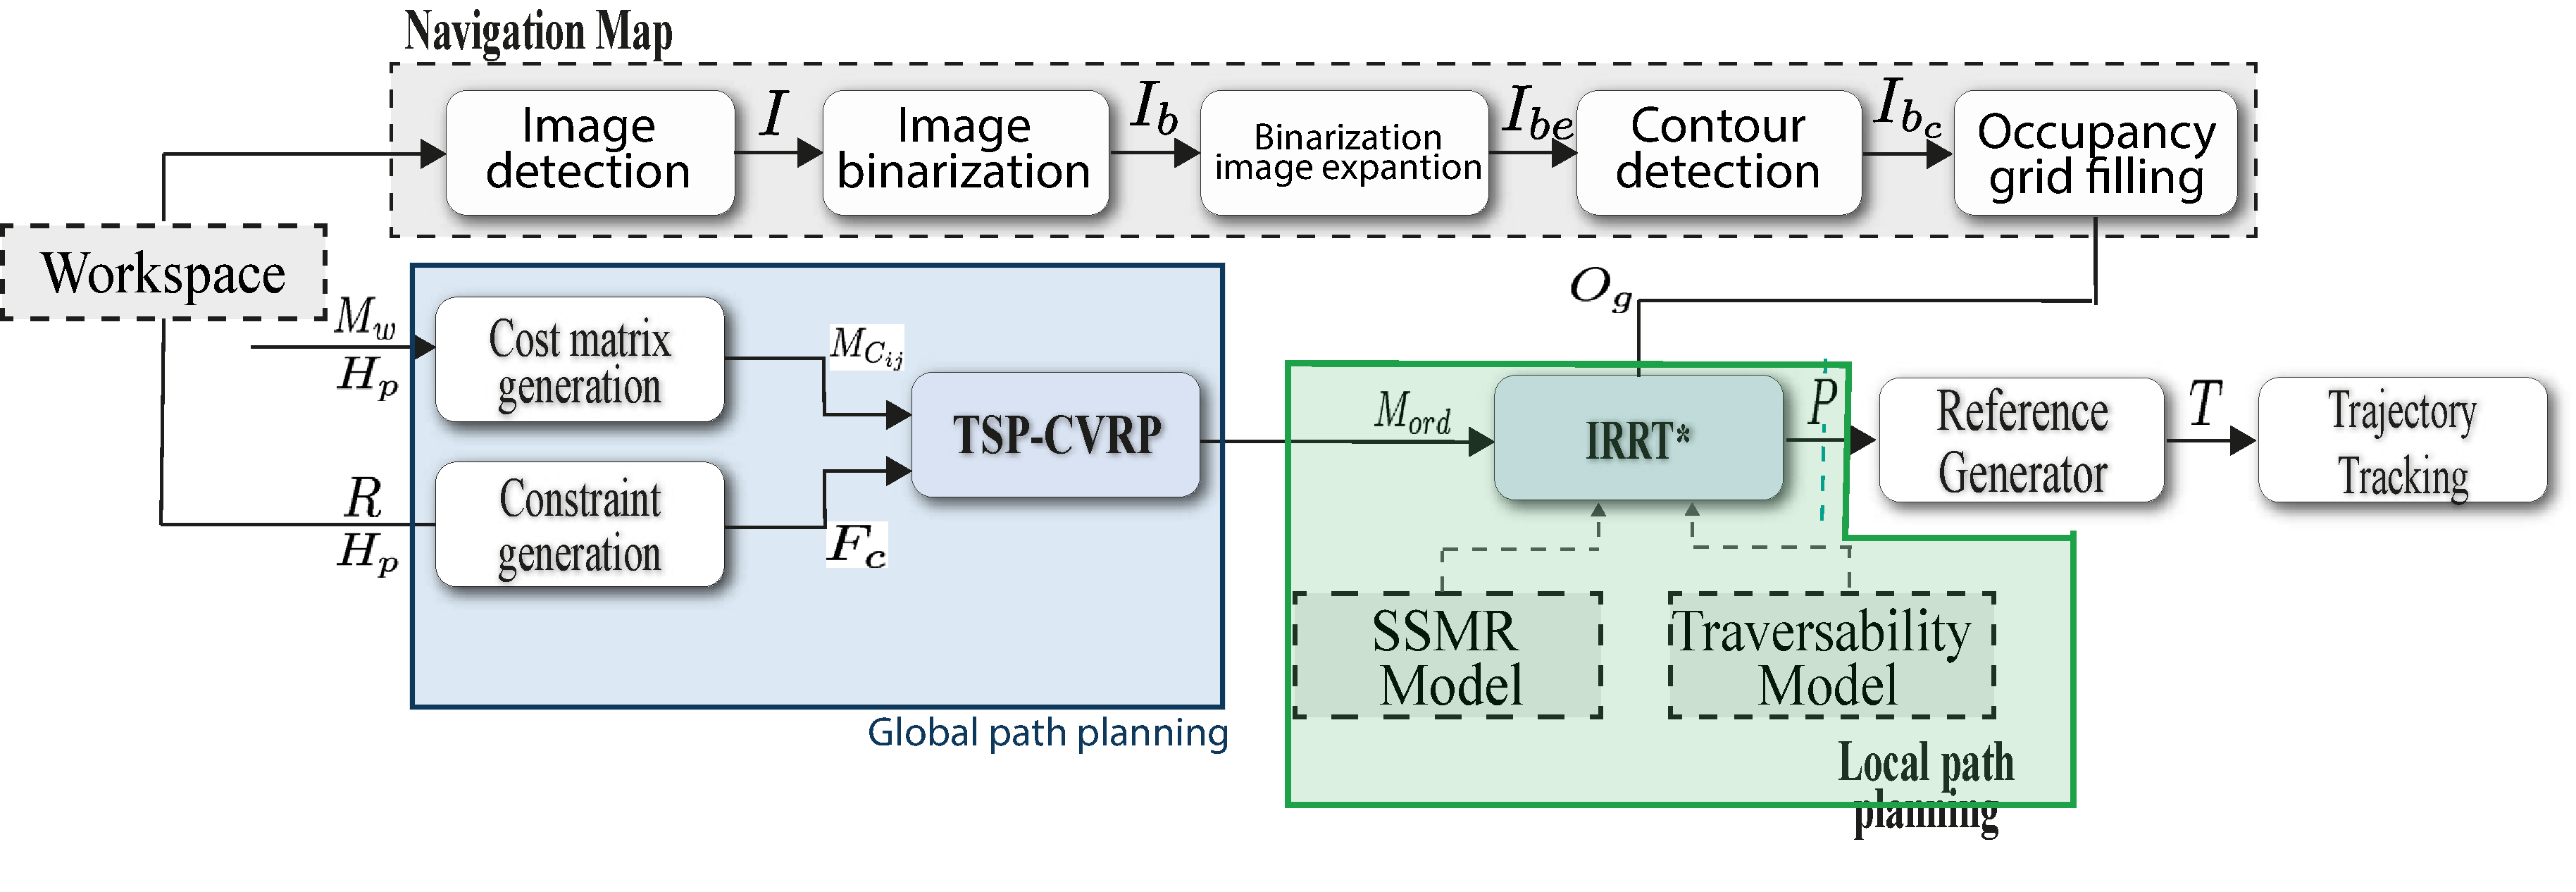
\includegraphics[width=\linewidth]{Images/methodology_5.pdf}
	\caption{General scheme of the integrated global and local planning strategy for SSMRs under terrain constraints.\revL{No entiendo como es que el global path planning obtiene la ubicacion de los puntos de recoleccion y las interconexiones entre ellos (edges). No deberia eso venir del navigation map?}}
	\label{Fig::esquema_basico_planificacion}
\end{figure*}


In addition, probabilistic methods such as RRT or PRM are commonly integrated with Unmanned Ground Vehicles (UGV) for spraying, planting, and harvesting \cite{Papadakis2013, ALMILLI2010151, Fernandez2019, Milos2022, Dereci2022}. In the same line of UGV this work uses the SSMR. SSMR is particularly favored in various off-road applications, including agriculture \cite{Dutta2019}, mining \cite{Szrek2022}, and foraging \cite{Auzan2022}, owing to its straightforward construction and remarkable flexibility. The maneuverability of a SSMR results from the variance in angular velocities between its right and left wheels \cite{Tagliavini2022}. In agricultural contexts, SSMRs prove advantageous due to their ability to navigate challenging terrains with ease, making them well-suited for tasks like precision planting and harvesting. The simplicity of their mechanical design ensures reliability in demanding environments, and their adaptability allows for seamless integration with local path planning techniques.

In \cite{Auat2017}, path planning strategy takes into account the robot's kinematic constraints while considering terramechanical limitations. This contribution presents an integrated strategy for harvest and motion planning, utilizing crop yield information. Harvesting locations are formulated as a Traveling Salesman Problem (TSP), while motion planning is addressed using the RRT* algorithm, which incorporates terrain traversability. However, this work raises some concerns: a) The cumulative effort savings was only 5\% when using RRT* using terrain constraints compared to the case of using RRT* without terrain constraints, b) The cumulative path-following error does not show a representative difference when using RRT* with and without terrain constraints. 

According to \cite{Xu2020}, the path calculation speed in RRT can be slowed down by the starting and ending point locations, size of the search configuration space, inefficient sampling, or new obstacles in the scene. To try to improve the speed, it was fusioned PRM and bidirectional RRT based on probability (P-Bi-RRT), which divides the planning area into two equally sized regions on average. The PRM algorithm with faster planning speed is used to prepare the route in each area, followed by selecting nodes from each region to generate an optimal pair of matching points. These points are then used to connect the two regional routes. Although the proposed integration of PRM and RRT in this work allows to reduce the planning time and path length. It does not consider the kinematics of some robot, which can cause that the path cannot be executed satisfactorily. 


One of the frequent problems in path construction with RRT algorithm is the efficiency of environment exploration with random points  \cite{Wang2022_Path}. For this reason, \cite{Chen2020} proposes a hybrid method of RRT with machine learning methods. This method uses a simultaneous generation process of a global tree and a local tree to explore the boundary points. The boundary points that are detected are filtered using the DBSCAN clustering method, from which a set of target points is obtained and used as the current target point for robot motion.


\textcolor{blue}{Most path planning works consider static and dynamic obstacles surrounding the vehicle, but few have taken into account the navigation terrain, which could be considered as the primary terra-mechanical constraint that affects the navigation performance through a reduced tractive force exertion and wheel slippage \cite{Prado2021}. Then, path planners that involves terrain traversability criteria to overcome complex terrain obstacles are more than welcome. For instance, considering terra-mechanical models of Hunt-Crossley in the design of a path planner allowed an autonomous ground vehicle to adapt a motion control to minimize the energy consumption based on different uneven and flexible navigation surfaces} \cite{10011864}. 


% \revJ{Esto debe ir en el contexto de planificadores de caminos y no como métodos aislados. Aqui ya se cambió de aplicación que tiene que ver con terra-mecánica, que es algo que nosotros no estudiamos}. Various empirical methods have been used to determine soil resistance, such as the cone index and maximum mean pressure \cite{ALMILLI2010151}. These methods offer a  evaluation mobility based on a "pass/fail" criterion. \revJ{Insisto, no necesitamos saber como se modela el terreno, sino como se usa el terreno en un planificador y que impacto pudo haber tenido si alguien lo hizo. Si alguien lo hizo, cual sería la diferencia con lo nuestro}. 

% Based onb\cite{Papadakis2013}, most empirical models were developed to assess soil penetration resistance. Papadakis points out two ways to estimate terrain traversability without physical interaction with the terrain \revJ{No poner esto en bullets}:

% \begin{enumerate}
%   \item Geometry-based (point clouds with LiDAR, elevation maps).
%   \item Appearance-based (RGB images, multi-spectral images).
% \end{enumerate}

% \revJ{Insisto, esto debe ir en el contexto de planificadores de caminos y no en el de terra-mecánica}. Various mathematical models are available to predict wheel-terrain interaction based on terrain properties and wheel characteristics. Some of the most common models are \revJ{No poner esto en bullets}:

% \begin{itemize}
%   \item Coulomb Model \cite{Ding}: Based on Coulomb's law to calculate the wheel-terrain friction force.
%   \item Spencer Model: Based on Mohr-Coulomb theory \cite{Massoudi} to calculate friction force based on soil tension.
% \end{itemize}

% \revJ{Enfáticamente insisto!. Solo hablar de trabajos que tengan relación con el suyo o debe darle un enfoque a su trabajo. Los modelos deben hablarse si fueron usados en un planificador de caminos, sino es así es mejor sacarlos. Por ejemplo, se usó el modelo de Bekker en un RRT pero la complejidad hace infactible la aplicación en linea. O, un modelo Wong se usó para insertar la resistencia del suelo en el planificador Fuzzy, pero solo fué usado en terreno arenoso. Si usted usa uno de esos modelos o uno similar es un buen punto en el que si hay que incluir, pero debe hablar de como otros autores usan tal vez de forma similar a lo que usted usará}. Each of these models has its own advantages and disadvantages in terms of precision and complexity. Most works studying soil properties rely on a set of tests proposed by Bekker \cite{bekker1956theory}, known as the Bevameter Technique, which led to the development of pressure-sinkage and traction-slippage relationship models. Wong further expanded these models to allow the prediction of track resistance, traction effort, and slip for a track based on soil properties \cite{Wong}.

% as shown in Equations 1 and 2 by \cite{ALMILLI2010151}

% \begin{equation}
% R_{c}=\dfrac{bl}{(n+1)(\dfrac{k_{c}}{b+k_{\phi}})} * (\dfrac{W}{bl})^{(\dfrac{n+1}{n})}
% \end{equation}

% \begin{equation}
% F=(A_{c}+W\tan(\phi))[1+\dfrac{k}{il}(1-e^{-(\dfrac{il}{K})})]
% \end{equation}

% where \(R_{c}\) represents road motion resistance due to soil compaction, and \(k_{c}\), \(k_{\phi}\), and \(n\) are the pressure sinkage parameters. \(W\) stands for vehicle weight, \(l\) and \(b\) denote the length and width of contact of the track, respectively. \(F\) represents total traction, \(A\) is the track contact area (\(A = b \cdot l\)), \(c\) is cohesion, \(\phi\) represents the friction angle, \(K\) is the shear modulus, and \(i\) is the longitudinal slip of the track. These models have been applied in various works, such as terrain traversability modeling through reinforcement learning incorporating exteroceptive and proprioceptive sensor data \cite{GanLu}, and terrain traversability analysis for unmanned ground vehicles \cite{Papadakis2013}. These works identify that the core of all these methodologies uses 3D terrain information acquired through light sensors, stereo range data, color images, or other sensor data, occasionally combined with static or dynamic modeling of vehicle-terrain interaction.

% \revJ{Un solo párrafo aislado que habla de una sola cita y sin contexto. Luego salta a una frase concluyente que no tiene relación a la cita previa}.
% In \cite{Milos2022}, a generalized exploration of unknown environments by autonomous mobile robots is conducted, where a robotic agent learns terrain traversability and constructs a spatial model of the environment. After reviewing the literature, it is found that \revJ{Esto es su percepción. Mejore su oración final} \sout{few works} conduct path planning considering both the robot's kinematic constraints and the terrain constraints encountered in agriculture.

% \revJ{Párrafo fuera de lugar}. There are various kinematic models developed for off-road vehicles. However, these models have been simplified into empirical formulas, rendering them useless for online predictions \cite{ALMILLI2010151}. 
% This work adopts the dynamics and kinematics models by Bekker and Wong \cite{bekker1956theory}, \cite{Wong} for predicting the traversability and maneuverability performance of Skid-Steer differential drive-type vehicles.

%%%%%%%%%%%%%%%%%%%%%%%%%%%%%%%%%%%%%%%%%%%%%%%%%%%%%%
\section{Motion models for harvesting tasks}
\subsection{Model of the Skid-Steer Mobile Robot}

In a SSMR, the driving wheels are on the same axis, and the robot moves in a 2D plane. The speed of each wheel is denoted as $v_{r}$ for the right wheel and $v_{l}$ for the left wheel. The distance between the two wheels is referred to as $L$. The robot has a position $x$, $y$, and an orientation angle $\theta$. The pose of the robot $\zeta$ in the global frame of reference could be represented by vectors and is given by Eq. \ref{Eq::pos}. The relationship between the wheel speeds and the linear and angular velocities of the robot is described in Eq. \ref{Eq::v}, \ref{Eq::w},\ref{Eq::kinematics} that describe how the wheel speeds ($v_{r}$ and $v_{l}$) translate into the linear velocity $v$ and angular velocity $\omega$ of the robot, which in turn affect the position and orientation of the robot over time  \cite{Prio2019,guevara2019}.

\begin{enumerate}
    \item Pose of the robot:
    \begin{equation} \label{Eq::pos}
    \zeta = \begin{pmatrix}
        x \\
        y \\
        \theta
    \end{pmatrix}
    \end{equation}
    \item Linear Velocity of the Robot:
    \begin{equation} \label{Eq::v}
        v = \frac{v_r + v_l}{2}
    \end{equation}
   
    \item Angular Velocity of the Robot:
    \begin{equation} \label{Eq::w}
    \omega = \frac{v_r - v_l}{L}
    \end{equation}
  
    \item Robot Kinematics: The change in the robot's position based on its linear and angular velocities is given by:  
    \begin{equation} \label{Eq::kinematics}
        \begin{split}
        \dot{x} &= v \cos(\theta) \\ 
        \dot{y} &= v \sin(\theta) \\
        \dot{\theta} &= \omega
    \end{split}
    \end{equation}
\end{enumerate}

\subsection{Model of the terrain traversability}
The Coulomb friction model \cite{Popov2017,Ding } describes the frictional force (\( F_{s} \)) between two surfaces as the product of the coefficient of friction ($\mu_{s}$) and the normal force (\( F_{s} \)). The model is represented by the Eq.\ref{Eq::columb}:

\begin{equation}
\label{Eq::columb}
 F_{s} = \mu_{s} \cdot F_{N} 
\end{equation}

\noindent where \( F_{s} \) is the frictional force, \( \mu \) is the coefficient of static friction, and \( F_{N} \) is the normal force, typically referring to the weight of the SSMR in static situations. This model assumes that the static and kinetic friction forces are equal until the applied force exceeds the product \( \mu \cdot F_{N} \), at which point sliding begins, and the friction force reaches its maximum value. The application of this model requires knowledge of the coefficient of friction (\( \mu \)) and the normal force (\( F_{N} \)). It is important to note that this model is a simplification, neglecting factors such as the relative velocity between surfaces and changes in surface characteristics.



\section{Prerequisites and methods applied}
\label{Sec::methdology}
The proposed work was developed through an experimental methodology to fulfill the specific objectives. Next, the proposed methodology follows 3 stages: first the image of the environment is processed, then a global path planning is generated by TSP-CVRP to then generate a local path with RRT*-Informed for the SSMR as shown in Fig. \ref{Fig::esquema_basico_planificacion}

\begin{table}[t!]
    \centering
    \caption{Abbreviations and Formulas \revR{aqui usted mezcla abreviatura con nomenclatura. ERROR}}
    \label{Table::abbreviations_continued}
    \begin{tabularx}{\columnwidth}{@{}clX@{}}
        \toprule
        \textbf{Abbreviation} & \textbf{Description} \\
        \midrule
        \textbf{$\epsilon$} & Incremental distance \\
        \textbf{$X$} & Configuration space of the vehicle \\
        \textbf{$z_{\text{init}}$} & Initial configuration of the robot \\
        \textbf{$z_{\text{rand}}$} & Randomly sampled configuration \\
        \textbf{$z_{\text{nearest}}$} & Nearest neighbor configuration to $z_{\text{rand}}$ \\
        \textbf{$z_{\text{new}}$} & New configuration added to the tree \\
        \textbf{$Z_{\text{nearTo}}$} & Configurations near $z_{\text{new}}$ \\
        \textbf{$Z_{\text{nearFrom}}$} & Configurations near $z_{\text{new}}$ for rewiring \\
        \textbf{$\text{Cost}(z)$} & Cost of reaching configuration $z$ \\
        & from the initial configuration  \\
        \textbf{$c(z_1, z_2)$} & Cost of transitioning from \\
        & configuration $z_1$ to $z_2$  \\
        \textbf{$P_i$} & Waypoints in the path \\
        \textbf{$S_i(x)$} & Cubic spline function between $P_i$ and $P_{i+1}$ \\
        \textbf{$O_{g}$} & Occupancy Grid \\
        \textbf{$I_{b}$} & Binarized Image \\
        \textbf{$I_{b_{e}}$} & Expanded Binarized Image \\
        \textbf{$C$} & Constant subtracted from the mean  \\
        & in Adaptive Thresholding \\
        \textbf{$b_{s}$} & Size of the local neighborhood \\
        & in Adaptive Thresholding  \\
        \textbf{$k$} & Kernel size for the median blur filter \\
        \textbf{$D_{ij}$} & Euclidean distance between two points \\
        \textbf{$w_{j}$} & Weight associated with $H_{p_{j}}$ \\
        \textbf{$Q$} & Maximum capacity of each vehicle \\
        \textbf{$H_{p}$} & Harvest points \\
        \textbf{$N$} & Total number of iterations \\
        \textbf{$L$} & Distance between the two wheels of the robot \\
        \textbf{$\theta$} & Orientation angle of the robot \\
        \textbf{$v_r$} & Speed of the right wheel \\
        \textbf{$v_l$} & Speed of the left wheel \\
        \textbf{$v$} & Linear velocity of the robot \\
        \textbf{$\omega$} & Angular velocity of the robot \\
        \bottomrule
    \end{tabularx}
\end{table}

\revL{En la Tabla 1 defines $v_r$ como Speed, no deberia ser Angular velocity?}
To obtain a navigation map to use in the local path planner a image is processed in 5 steps. Initially, a vision sensor captures an image, which is then subjected to background removal to isolate relevant features. The image is subsequently converted to an binarized image $\mathcal{I}_{b}$. Then a median blur operation is applied, which can be expressed as: $\mathcal{I}_{b} = \text{MedianBlur}(O_{g}, k)$ where $k$ represents the kernel size for the median blur filter. Then, an adaptive thresholding is used to binarize the blurred image. This operation can be described as: $\mathcal{I}_{b} =\text{AdaptiveThreshold}(\mathcal{I}_{b}, b_{s}, C)$ where $\mathcal{I}_{b}$ represents the binary image, $b_{s}$ is the size of the local neighborhood, and $C$ is a constant subtracted from the mean.  The $\mathcal{I}_{b}$ is subsequently expanded by aplying the method $\text{AdaptiveThreshold}$ process a binary occupancy grid, expanding safe navigation areas. By detecting contours and applying a large block size in the adaptive thresholding, the method identifies obstacles and sets corresponding regions in the occupancy grid to zero, effectively creating a safety margin around obstacles, resulting in $\mathcal{I}_{b_{e}}$. As the $\mathcal{I}_{b_{e}}$ is represented in obstacle and non-obstacle spaces, all rectangular contours of the obstacles on the map are detected. The subsequent step to fill the contour areas was aplied to enhance obstacle detection and ensure a comprehensive representation of obstacle regions in the occupancy grid. Leveraging the contours previously identified, the function calculates their areas and, based on a specified threshold (e.g., 40000), filters out smaller contours, effectively ignoring noise or insignificant details. The bounding rectangles of the retained contours are then used to modify the occupancy grid, setting the corresponding regions to zero, signifying obstacles. Additionally, the function visually highlights the identified obstacles by drawing rectangles on a copy of the input image. The resulting $\mathcal{I}_{b_{e}}$ encapsulates a refined representation of the environment, where all detected obstacle areas are accurately filled, mitigating the risk of false positives during path planning using the RRT algorithm. As a result of these 5 operations an Occupancy Grid $O_{g}$ is generated as shown in Fig. \ref{fig:rgb1}. 

The $O_{g}$ is a common discreet representation used in robotics and autonomous navigation \cite{ijgi11040231}. It is a discretized map of the environment, which is divided into a grid of cells. Each cell in the grid represents a small region in the physical world and marking them as occupied or free, the robot can efficiently navigate through complex spaces and avoid collisions. The purpose of an occupancy grid is to model whether these regions are occupied or free.  $O_{g}$ can be defined as a 2D matrix with binary values, where each element $O_{g(i, j)}$ indicates whether the corresponding cell is occupied (1) or free (0) where $i$ and $j$ are the row and column indices in the grid, respectively. 


\begin{figure*}[t!]
    \centering
    \includegraphics[width=\linewidth]{Images/image_process_6.pdf}
    \caption{Image processing to generate an $O_{g}$ with safe navigation limits for the robot. }
    \label{fig:rgb1}
\end{figure*}

\subsection{Global path planning}
\label{Subsec::global_path_planning}

To obtain an orderly harvesting route considering the maximum load capacity of the vehicle and the amount of product to be harvested in each row, the Capacitated Vehicle Routing Problem (CVRP) is used as shown in Algorithm \ref{Alg::TSP}. TSP-CVRP can be defined as a graph $G = (N, E)$, where $N$ is the set of ordered Harvest points $H_p = \{h_0, h_1, . . . , h_{mp}\}$, being $h_{0}$ the initial crop depot and $h_{mp}$ is the end crop point. Each edge $\{i, j\} \in E$ is associated with a non-negative cost. Each cost $C_{ij}$ is computed as follows:
\begin{equation}
C_{ij} = \frac{D_{ij} \times f_{w}}{w_{j} }    
\end{equation}
\noindent where $D_{ij}$ is the Euclidean distance that can be represented by $D_{ij} = \sqrt{(x_i - x_j)^2 + (y_i - y_j)^2}$; $f_{w}$ is an introduced factor that extrapolates distance between two latent harvesting points, which lie on two resident row sides, prioritizing a reduced-distance connection between harvesting points rather than forcing a direct connection. 


is a factor of navigation between rows, when the next $H_{p}$ to visit is in the same row the factor is 1 and if the next  $H_{p}$  to visit is in a different row the factor is 2, and $w_{j}$ is the amount of product in kilograms to be picked up at each $H_{p}$.

Every $H_{p}$ $i \in V' = V \setminus \{0\}$ has a specific demand $q_i$, where $i = 1, 2, . . . , n$. A single depot, denoted as $0$, dispatches one vehicle $K$, it has a limited load capacity $Q$. This vehicle departs from the depot or from one $H_{p}$ selected to serve each $H_{p}$ and then return to the depot. It's essential to note that the loading of each vehicle should not surpass the specified capacity limit $Q$. The main objective is to determine the a route to fulfill all $H_{p}$ demands while minimizing the total routing cost. The TSP-CVRP can be mathematically formulated as shown in Eq. \ref{Eq::TSP-CVRP}.

\begin{align}
\label{Eq::TSP-CVRP}
\notag \text{Minimize:} & \ \\
& \sum_{i=1}^{n}\sum_{j=1}^{n} C_{ij} x_{ij} \ \\
\notag \text{Subject to:} & \ \\
& \notag \sum_{j=1}^{n} x_{ij} = 1 \quad \forall i = 1, 2, ..., n \ \\
& \notag \sum_{i=1}^{n} x_{ij} = 1 \quad \forall j = 1, 2, ..., n \ \\
& \notag \sum_{j=1}^{n} w_j x_{ij} \leq Q \quad \forall i = 1, 2, ..., n \ \\
& \notag x_{ij} \in {0, 1} \quad \forall i, j = 0, 1, 2, ..., n \ \\
& \notag x_{ij} = 0 \quad \forall (i,j) \notin C \
\end{align}

\noindent where $C_{ij}$ represents the cost to travel between  $H_{p_{i}}$  and $H_{p_{j}}$ .
$x_{ij}$ is a binary variable indicating whether there is travel from  $H_{p_{i}}$  to $H_{p_{j}}$.
$w_{j}$ is the weight associated with $H_{p_{j}}$.
$K$ is the available vehicle.
$Q$ is the maximum capacity of each vehicle.
$C$ is the set of connections between specific $H_{p}$ that must be adhered to.

The TSP-CVRP operates on various input parameters, including matrices of $H_{p}$ denoted as $M_{p}$ and weights $M_{w}$ associated with each $H_{p}$, the maximum vehicle capacity $Q$, and a list of rows from the harvesting map $R$. \revL{Esto es justamente lo que no me quedo claro de la Fig.1, porque $M_{p}$, $M_{w}$ y $F_{c}$ no son producto de tu proceso de mapeo? como sabes las ubicaciones de los puntos de cosecha sin conocer el mapa? Hay que aclarar esto. i.e. por que cierta informacion del entorno debe ser procesada mientras que otra ya se la tiene?} The algorithm \ref{Alg::TSP} initializes and retrieves essential data, including the environment data, distance matrix $M_{c_{ij}}$, and forbidden connections matrix $F_{c}$. In order to adapt the TSP-CVRP optimization for agricultural environments, a method for generating forbidden connections $F_{c}$ between $H_{p}$ is applied. This method aims to prevent connections between each $H_{p}$  located in different rows and is represented through mathematical formulas and variables as follows:

Let $n$ represent the total number of rows in the agricultural layout, denoted as $h_{1}, h_{2}, \ldots, h_{n}$. For each row $h$ within the range $[2, n-1]$ and for each $H_{p}$ in the current row, denoted as $(H_{p_{n}}, H_{p}, H_{i})$, a set of conditions is applied to identify $H_{p}$ in adjacent rows. For the rows immediately above and below, denoted as $(h-1)$ and $(h+1)$, the method checks for the presence of $H_{p}$ in those rows. If such $H_{p}$ are found, a forbidden connection between the $H_{p}$ representing these $H_{p}$ is established, and this connection is recorded in the $F_{c}$ list as shown in Alg. \ref{Alg::forbidden_c}.

\begin{algorithm}[t!]
\caption{Get Forbidden Connections}
\label{Alg::forbidden_c}
\begin{algorithmic}[1]
\Require
\State $Rows \gets$ Dictionary of rows and objects
\State $F_{c} \gets$ Matrix of forbidden connections
\Ensure
\State \textbf{Initialize} $F_{c}$ as an empty list
\State \textbf{Initialize} $N_{r}$ as the length of $R$
\For{$h \gets 1$ to range($N_{r}$)}
    \State \textbf{Initialize} $C_{r} \gets$ $R$[h] \Comment{Current row}
    \State \textbf{Initialize} $P_{r} \gets$ $R$[h-1] \Comment{Previous row}
    \State \textbf{Initialize} $N_{r} \gets$ $R$[h+1] \Comment{Next row}
    \For{$Name, (H_{p},{H_{i}})$ in $C_{r}$}
        \If{'c' in $Name$}
            \If{$P_{r}$} \Comment{Find the centers of each row}
                \For{$P_{on}$, ($P_{o_{p}}$, $P_{o_{i}}$) in $P_{r}$}
                    \State $F_{c} \gets$ $H_{i}$, $P_{oi}$ \Comment{Store the current object and the object from the next row meeting the condition, e.g., (2,6)}
                \EndFor
            \EndIf
            \If{$N_{r}$}
                \For{$N_{on}$, ($N_{op}$, $N_{o_{i}}$) in $P_{r}$}
                    \State $F_{c} \gets$ $H_{i}$, $N_{o_{i}}$
                \EndFor
            \EndIf
        \EndIf
    \EndFor
\EndFor
\State \textbf{Return} $F_{c}$
\end{algorithmic}
\end{algorithm}

Once the TSP-CVRP constraints have been generated, the TSP-CVRP algorithm starts at the depot $M_{p}[0]$ and explores unvisited $H_{p}$ to create a solution. It uses the Path Cheapest Arc strategy to find the nearest unvisited $H_{p}$  $M_{p}[i+1]$ from the current $H_{p}$  $M_{p}[i]$. It checks if there are any forbidden connections $F_{c}$ between $H_{p}$ and ensures that the weight of the collection $S_{w}$ does not exceed the vehicle's capacity $Q$. If these conditions are met, the algorithm proceeds to create a solution $S$. The process continues until all $H_{p}$ are visited. Finally, the algorithm applies a Tabu Search algorithm to obtain an ordered matrix of $H_{p}$ positions $M_{ord}$ for efficient routing as shown in Algorithm \ref{Alg::TSP}.

\begin{algorithm}[t!]
\caption{TSP-CVRP}
\label{Alg::TSP}
\begin{algorithmic}[1]
\Require
\State $O_{g} \gets$ Occupancy Grid
\State $M_{p} \gets$ Visiting $H_{p}$  Matrix
\State $M_{w} \gets$ Matrix of weights
\State $Q \gets$ Maximum vehicle capacity
\State $Rows \gets$ Dictionary of rows and objects
\Ensure
\State Ordered matrix of visiting $H_{p}$  positions
\State \textbf{Initialize} $Data $ = getDataEnvironment() \Comment{Retrieve positions, weights, and rows of the objects}
\State \textbf{Initialize} $D_{m} $ = getDistances($Data$) \Comment{Obtain distance matrix}
\State \textbf{Initialize} $F_{c} $ = getForbiddenConnections($R$) \Comment{Obtain restrictions matrix}
\State \textbf{Initialize} $S_{w} \gets$ 0 \Comment{Collection sum}
\State Start at $M_{p}[0]$ and mark all $M_{p}[i]$ as unvisited
\While{there are to visit}
\State \textbf{Apply} PCA  \Comment{Obtain the first solution}
\State Find the nearest $M_{p}[i+1]$ to the current $M_{p}[i]$ that has not been visited yet.
\If{$M_{p}[i+1]$ and $M_{p}[i]$ are not in $F_{c}$}
\If{$S_{w} \leq Q$}
\State Go to the nearest $M_{p}[i]$ and mark the current $M_{p}[i]$ as visited.
\State $S_{w} \gets$ sum of $M_{w}[i]$
% \State $S \gets$ \textbf{PATHCHEAPESTARC} \Comment{Obtain the first solution}
\EndIf
\EndIf
\EndWhile
\State $M_{ord} \gets$  \textbf{TS(S)} \Comment{Ordered matrix of $H_{p}$}
\end{algorithmic}
\end{algorithm}

\subsection{Local path planning}
\label{Subsec::global_path_planning}
Once an ordered list $M_{ord}$ from TSP-CVRP is obtained a local path planner is used to find a local path where the robot can navigate safely avoiding obstacles and possible slippage areas. To improve this a IRRT$^*$ is used integrating SSMR Model. The integrated algorithm, is presented in Alg. \ref{Alg::rrt-unycle}. The algorithm is designed to find a feasible path for a SSMR from a given start state to a multiples goals states. The algorithm operates in an environment represented by an $O_{g}$. This algorithm combines the principles of RRT*-Informed for efficient exploration and the integration the SSMR model to ensure that the generated paths are feasible for the robot. RRT* \cite{Qi2021} is an incremental, sampling-based planner with guaranteed asymptotic optimally, originally developed for holonomic systems. The algorithm \ref{Alg::rrt-unycle},  is an extension of RRT* for SSMR. It solves the path planning problem by growing a tree $T = (V, E)$ with a vertex set $V$ of poses connected by edges $E$ of feasible path segments to find a path that connects exactly to the destination pose with minimum cost, using a set of basic procedures described below. $X$ is the configuration space of the vehicle, and $x: [0, 1] \to X$ is a path in the configuration space. The notations generally follow the RRT* algorithm are presented in \cite{Qi2021}. Where is characterized by the following functions: i) The sampling process samples a pose $z_{\text{rand}} \in X_{\text{free}}$ from the obstacle-free region of the configuration space. The sampling is random with a goal bias, with which the destination pose is sampled to ensure that the path exactly connects to the destination pose. 
\revR{Falta completar la descripccion del RRT en base a los cambios que se realizaran con la integracion del modelo}

The generation of a navigation area instead of a single navigation path is done by means of a function that evaluates collision conditions between two nodes, taking into account both the collision along the line segment between the nodes and potential obstacles within a circular area of radius $r$ around the second node. It is defined as follows:
\begin{equation}
\forall (x, y) \in \text{Circular Area}\, : \, O_{g}[\lfloor x \rfloor][\lfloor y \rfloor] \neq 0 
\end{equation}

\noindent where the "Circular Area" is defined by \( (x - x_2)^2 + (y - y_2)^2 \leq r^2 \), where \( (x_2, y_2) \) represents the coordinates of the second node.

\begin{figure}[t!]
        \centering
        \includegraphics[width=\linewidth]{Images/collision_2.pdf}
        \caption{Collision and traction terrain detection}
        \label{fig:collision}
\end{figure}

In the path planning process, the generated path from the RRT-Star algorithm may exhibit sharp turns and jagged edges, making it suboptimal for robot navigation. To address this, piecewise cubic polynomial interpolation is employed using the CubicSpline function from \cite{scipy}. The key idea is to fit a cubic polynomial between each pair of consecutive waypoints, creating a smooth trajectory. Let $P_{i}$ represent the waypoints in the path, and $S_{i}(x)$ be the cubic spline function between $P_{i}$ and $P_{i+1}$. The CubicSpline algorithm determines the coefficients $a_{i}, b_{i}, c_{i}, d_{i}$ for each segment, resulting in a continuous and differentiable curve. The interpolated path is then obtained by evaluating the spline functions over a finer resolution. This process could ensures a kinematically feasible trajectory for the robot. $S_{i}(x)$ is defined as Eq. \ref{Eq::cubic}:

\begin{equation}
\label{Eq::cubic}
S_{i}(x) = a_{i}(x - P_i)^3 + b_{i}(x - P_i)^2 + c_{i}(x - P_i) + d_{i}
\end{equation}

\noindent where \(P_i\) represents the ith waypoint, and \(a_i, b_i, c_i, d_i\) are the computed coefficients. This interpolation enhances the path quality, providing a more suitable trajectory for robotic navigation.

\begin{algorithm}[t!]
\caption{ $T =(V,E) \leftarrow$RRT* Informed for the SSMR}
\label{Alg::rrt-unycle}
\begin{algorithmic}[1]
\State $T  \leftarrow$ InitializeTree();
\State $T \leftarrow$ InsertNode$(\emptyset, z_{\text{init}}, T)$;
\For{$i = 1$ to $N$}
    \State $z_{\text{rand}} \leftarrow$ Sample$(i)$;
    \State $z_{\text{nearest}} \leftarrow$ Nearest$(T, z_{\text{rand}})$;
    \State $(z_{\text{new}}, x_{\text{new}}) \leftarrow$ Extend$(z_{\text{nearest}}, z_{\text{rand}}, \epsilon)$;
    \If{ObstacleFree$(x_{\text{new}})$}
        \State $Z_{\text{nearTo}} \leftarrow$ NearTo$(T, z_{\text{new}, |V|})$;
        \State $z_{\text{min}} \leftarrow$ ChooseParent$(Z_{\text{nearTo}}, z_{\text{nearest}}, z_{\text{new}})$;
        \State $T \leftarrow$ InsertNode$(z_{\text{min}}, z_{\text{new}}, T)$;
        \State $Z_{\text{nearFrom}} \leftarrow$ NearFrom$(T, z_{\text{new}, |V|})$;
        \State $T \leftarrow$ ReWire$(T, Z_{\text{nearFrom}}, z_{\text{min}}, z_{\text{new}})$;
    \EndIf
\EndFor
\State \textbf{return} $T$
\end{algorithmic}
\end{algorithm}

\begin{algorithm}[t!]

\caption{$z_{\text{min}} \leftarrow$ ChooseParent( $Z_{nearFrom}$,  $Z_{nearest}$,  $Z_{new}$)}
\label{Alg::ChooseParent}
\begin{algorithmic}[1]
\State $z_{\text{min}} \leftarrow z_{\text{nearest}};$
\State $c_{\text{min}} \leftarrow \text{Cost}(z_{\text{nearest}}) + c(z_{\text{nearest}}, z_{\text{new}});$
\For{$z_{\text{near}} \in Z_{\text{nearTo}}$}
    \State $x_0 \leftarrow \text{Steer}(z_{\text{near}}, z_{\text{new}});$
    \If{ObstacleFree($x_0$)}
        \State $c_0 \leftarrow \text{Cost}(z_{\text{near}}) + c(z_{\text{near}}, z_{\text{new}});$
        \If{$c_0 < \text{Cost}(z_{\text{new}})$ and $c_0 < c_{\text{min}}$}
            \State $z_{\text{min}} \leftarrow z_{\text{near}};$
            \State $c_{\text{min}} \leftarrow c_0;$
        \EndIf
    \EndIf
\EndFor
\State \textbf{return} $z_{\text{min}};$
\end{algorithmic}
\end{algorithm}

\begin{algorithm}[t!]
\caption{$T \leftarrow$ ReWire($T$, $Z_{nearFrom}$, $z_{min}$, $z_{new}$)}
\label{Alg::ReWire}
\begin{algorithmic}[1]
\For{$z_{\text{near}} \in Z_{\text{nearFrom}} \setminus \{z_{\text{min}}\}$}
    \State $x_0 \leftarrow \text{Steer}(z_{\text{new}}, z_{\text{near}});$
    \If{ObstacleFree($x_0$) and Cost($z_{\text{new}}$) + $c(z_{\text{new}}, z_{\text{near}}) < \text{Cost}(z_{\text{near}})$}
        \State $T \leftarrow \text{ReConnect}(z_{\text{new}}, z_{\text{near}}, T);$
    \EndIf
\EndFor
\State \textbf{return} $T;$
\end{algorithmic}
\end{algorithm}


\subsection{Trajectory Tracking}
\section{Results and analysis}
\label{Sec::results}
This section presents the experimental setup and results of the proposed algorithm.

\subsection{Setup experimental}

These field tests were performed by the construction of a 3D map within Coppelia V-REP \cite{Ramin2018} simulating multi-row crop. In the conducted experiments, a 15 x 15-meter map was build, comprising 6 collection rows. Each row has a width of 4 meters and a length of 3 meters and Each collection row features a designated waypoint to which the robot is tasked to navigate for crop harvesting.  

\subsection{Assessment of harvest location priorization}

\label{Sec::test1}
\revJ{Se pide una prueba que planifique ruta para la recolección de producto bajo diferentes condiciones de punto inicio-fin, capacidades de carga, durante una operación de cosecha. Aqui se debe comparar caulitativamente los resultados con las tres estrategias de planificación. Para ello, genere estadísticas.}.

\begin{figure*}[t!]
    \begin{minipage}{1\textwidth}
        \centering
        \includegraphics[width=\linewidth]{Images/tsp_1.pdf}
        \caption{Assessment results comparing $H_{p}$ prioritization based on maximum payload capacity versus the proximity between harvest locations. The first row displays outcomes where the starting point corresponds to the endpoint, while in the second row, the starting and endpoint may not necessarily match. } 
        \label{fig:tsp_tests}
    \end{minipage}\hfill
\end{figure*}


\subsection{Path planning tests with terrain disturbances}
\label{Sec::test2}
\revJ{Se pide una prueba que planifique un camino durante una operación de cosecha sujeta a perturbaciones de terreno. Aqui se debe comparar cuantitativamente los resultados con las tres estrategias de planificación. Para ello, genere estadísticas}.


\begin{figure}[t!]
        \centering
        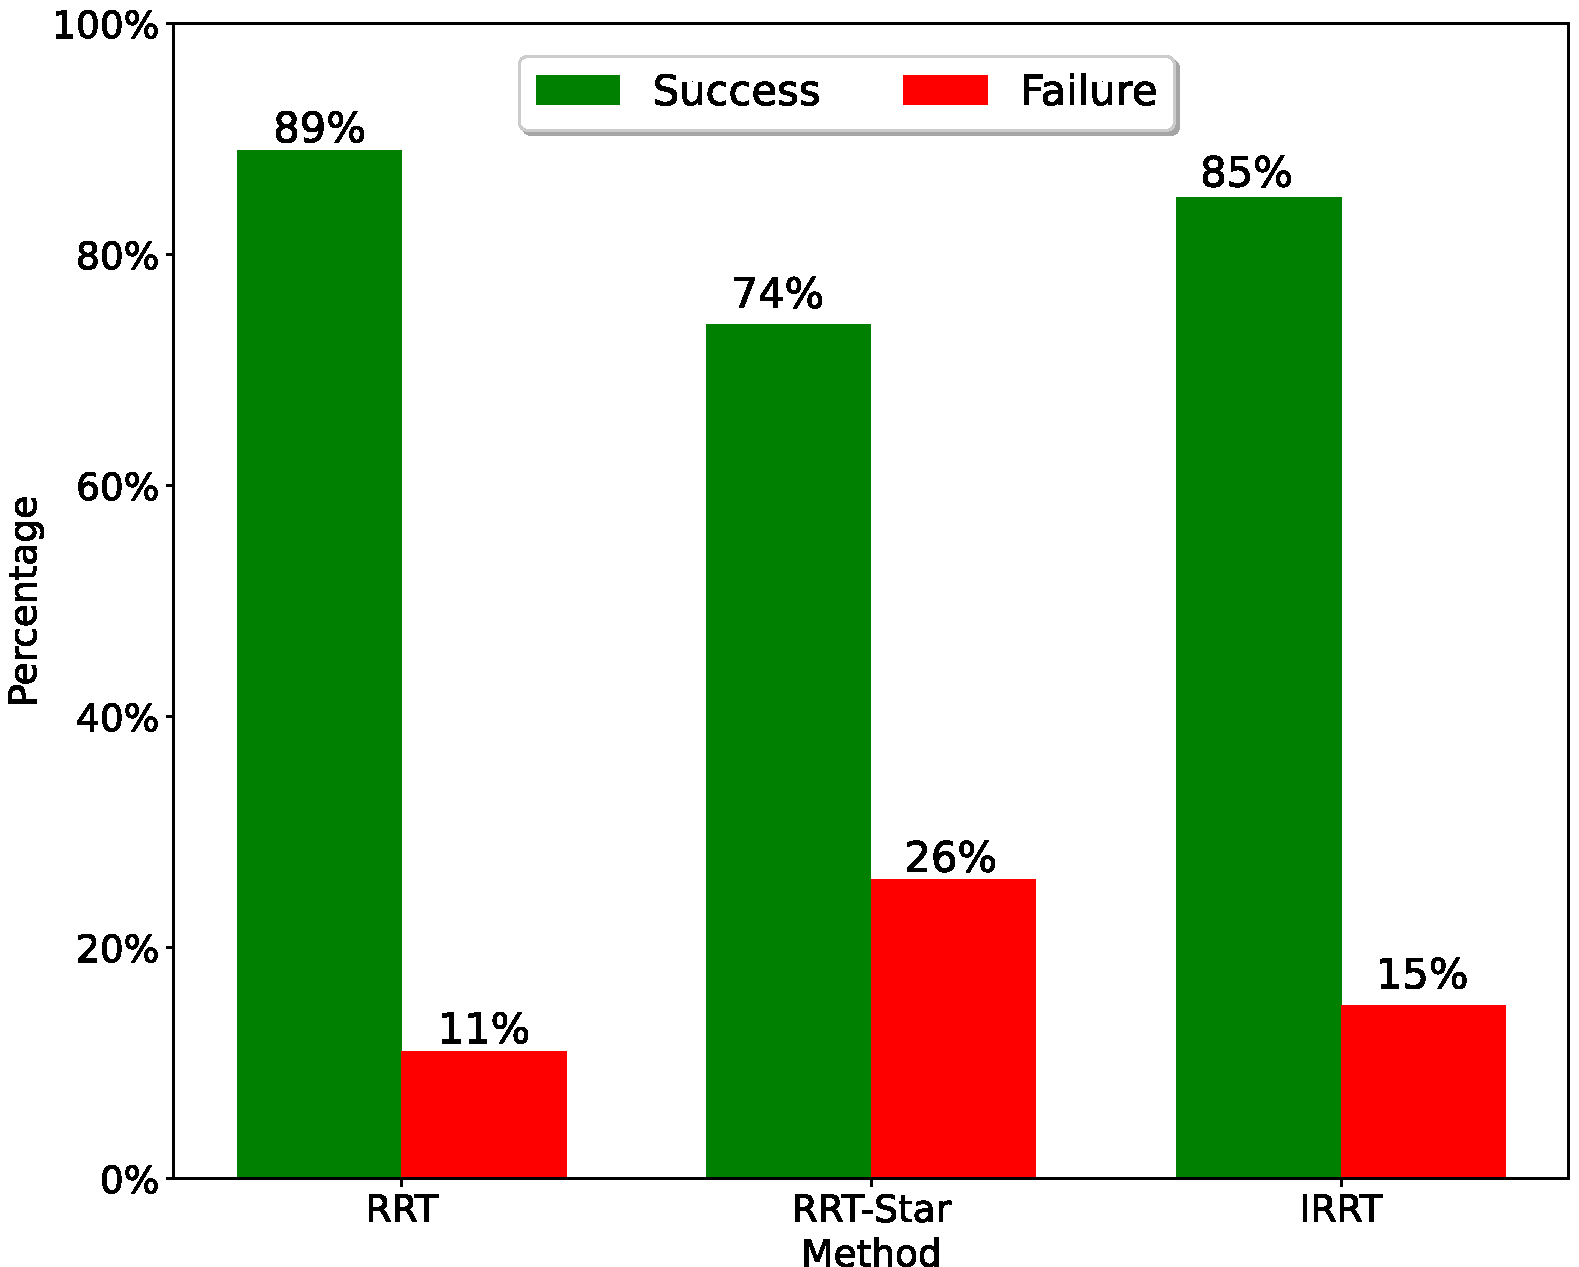
\includegraphics[width=\linewidth]{Images/rate_success_rrt_1.pdf}
        \caption{Success failure rate by method}
        % Test 20231210-aea28ef2-3437-424e-afc1-63fd1a8cc230
        \label{fig:test_rrt}
\end{figure}

\begin{figure}[t!]
        \centering
        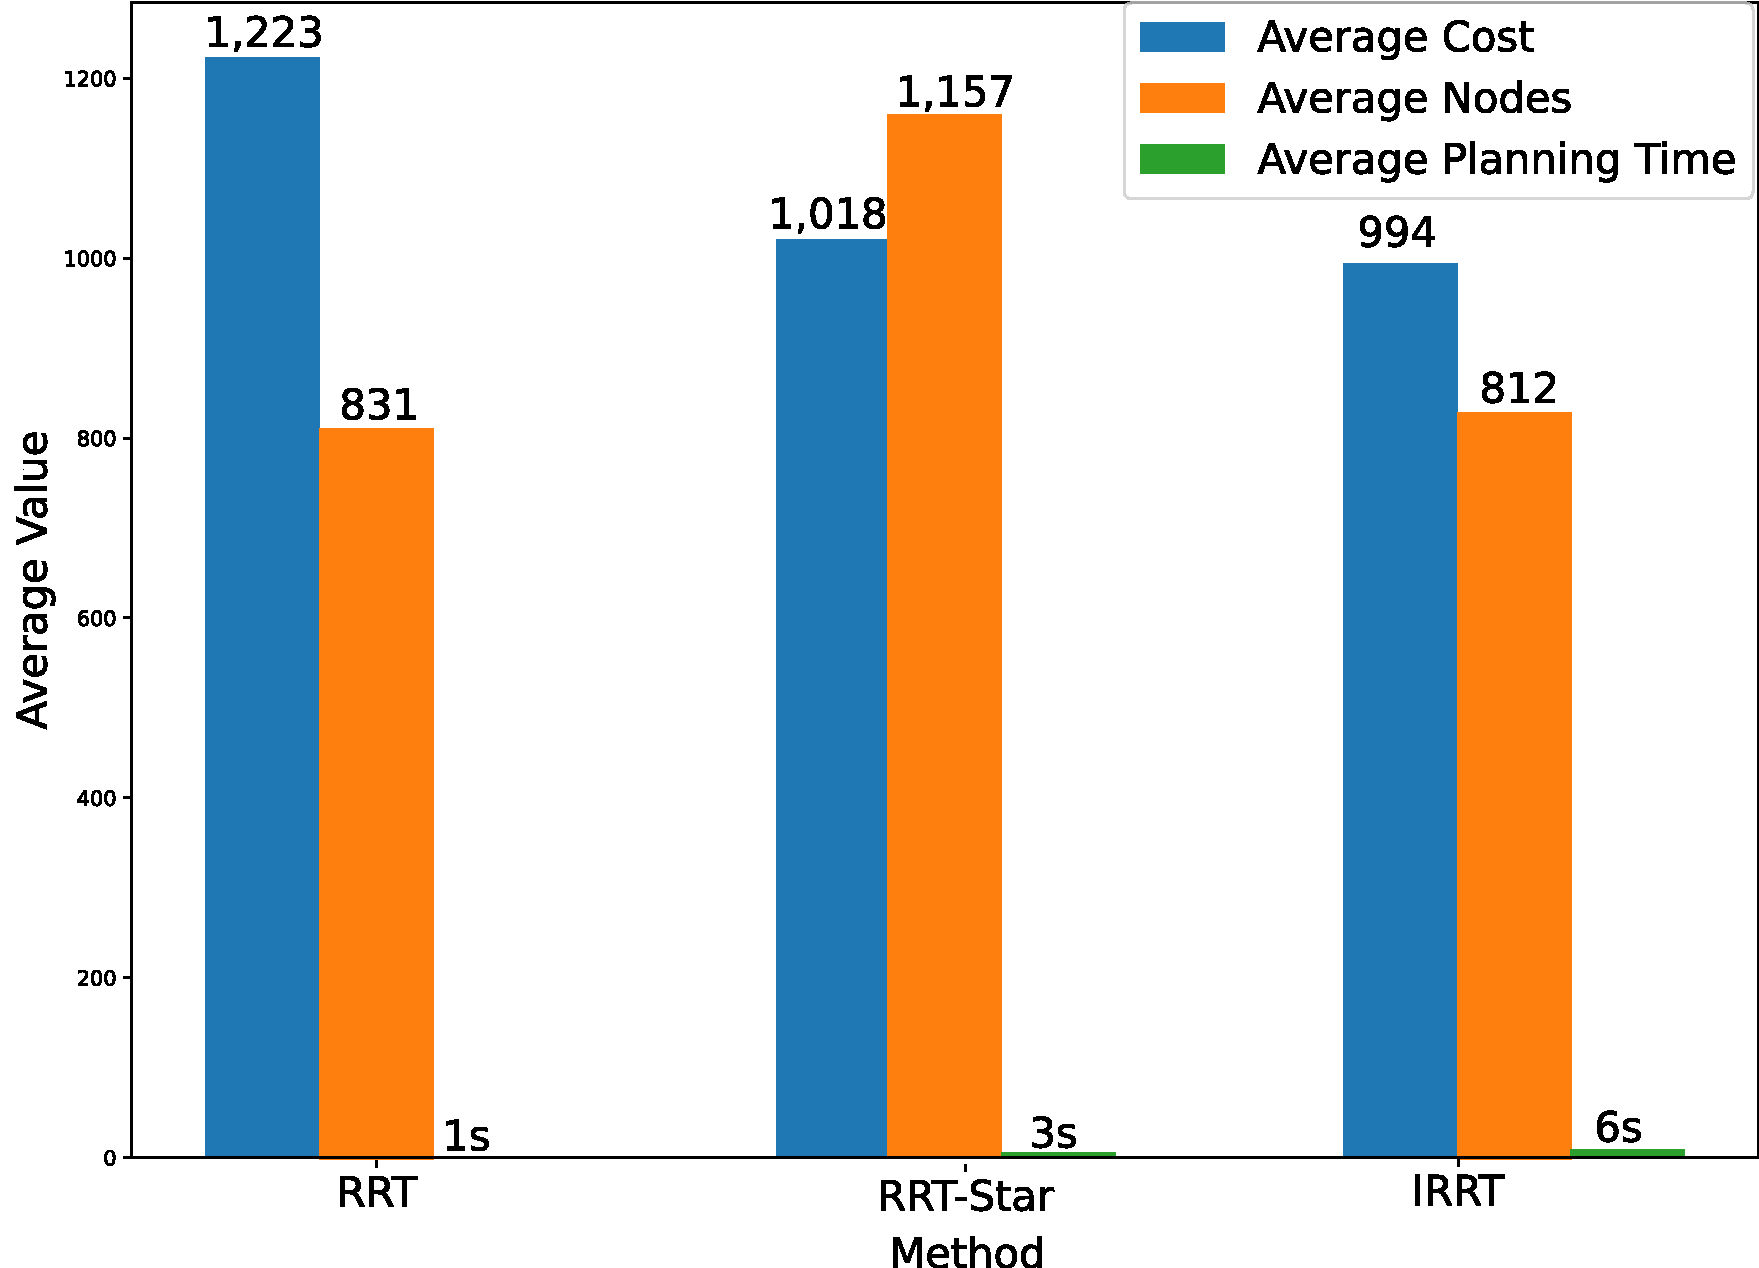
\includegraphics[width=\linewidth]{Images/report_rrt_1.pdf}
        \caption{Average Metrics for Successful Tests by Method of 50 Experiments}
        \label{fig:test_rrt}
\end{figure}

\begin{figure}[t!]
        \centering
        \includegraphics[width=\linewidth]{Images/test_rrt_5.pdf}
        \caption{Differences between RRT, RRT*, and IRRT*}
        \label{fig:test_rrt}
\end{figure}

\begin{figure}[t!]
        \centering
        \includegraphics[width=\linewidth]{Images/tsp_rrt_1.pdf}
        \caption{TSP and IRRT*}
        \label{fig:test_rrt}
\end{figure}

\begin{figure*}[t!]
    \centering
    \includegraphics[width=\linewidth]{Images/rrt_all_tests_2.pdf}
    \caption{Multiple test IRRT }
    \label{fig:rgb1}
\end{figure*}

\begin{figure*}[t!]
    \centering
    \includegraphics[width=\linewidth]{Images/rrt_all_tests_3.pdf}
    \caption{Multiple test IRRT }
    \label{fig:rgb1}
\end{figure*}

\begin{figure*}[t!]
    \centering
    \includegraphics[width=\linewidth]{Images/rrt_all_tests_4.pdf}
    \caption{Multiple test IRRT }
    \label{fig:rgb1}
\end{figure*}

\begin{table}[t!]
\centering

\caption{COMPARISON OF EXPERIMENT DATAS (DATAS ARE THE AVERAGE OF 100 EXPERIMENTS)}
\label{Table::results_rrt}
\begin{tabular}{@{}ccllcllccccc@{}}
\toprule
\multicolumn{1}{l}{\textbf{Algorithm}} & \multicolumn{3}{c}{\textbf{Pl(px)}} & \textbf{Cost} & \multicolumn{3}{c}{\textbf{Nnt}} & \textbf{Nn} & \textbf{Sr}  & \textbf{Pt(s)} \\ \midrule \midrule
\textbf{RRT} & \multicolumn{3}{c}{1} & \multicolumn{3}{c}{1} & 1 & 1 & 1 & 1\\
\textbf{RRT*} & \multicolumn{3}{c}{1} & \multicolumn{3}{c}{1} & 1 & 1 &  1 & 1 \\
\textbf{RRT* Informed} & \multicolumn{3}{c}{1} & \multicolumn{3}{c}{1} & 1 & 1  & 1 & 1 \\ 
\textbf{RRT* for SSMR} & \multicolumn{3}{c}{1} & \multicolumn{3}{c}{1} & 1 & 1 & 1 & 1 \\ \bottomrule
\end{tabular}
\end{table}

\subsection{Assessment of trajectory tracking performance}
\label{Sec::test3}

\revJ{Se pide una prueba que siga una trajectoria planificada durante una operación de cosecha sujeta a perturbaciones de terreno. Aqui se debe comparar cuantitativamente los resultados con las tres estrategias de planificación. Para ello, genere gráficas comparativas de al menos error acumulado, esfuerzo de control y costo total}.

\section{Conclusions}
\label{Sec::conclusions}

\section*{Acknowledgment}
The authors thank the support of ANID under Fondecyt Iniciaci\'on en Investigaci\'on 2023 Grant 11230962. It is also acknowledged the support of UCN under project 202203010029 -VRIDT-UCN, AC3E (ANID/ BASAL/FB0008), Anillo de Investigación en Ciencia y Tecnología -ACT210052, and Fondef IDEA I+D 2021 Cod. ID21 $\vert$ 10181.

\bibliographystyle{IEEEtran}
\bibliography{BIB}
\vspace{12pt}

\end{document}
